\documentclass[tikz,border=0mm]{standalone}
\usepackage[utf8]{inputenc}
\usepackage{unicode-math} % for unicode support in math environments
\usepackage{amsmath}
\usepackage{siunitx}
\usepackage{booktabs}
\sisetup{mode=text,range-phrase = {\text{~to~}}, range-units=single, print-unity-mantissa=false}
\usepackage{mhchem}
\usepackage{tikz}



\usepackage{fontspec}

\directlua{
  luaotfload.add_fallback(
  "FallbackFonts",
  {
        "DejaVu Serif:mode=harf;",
        "DejaVu Sans Mono:mode=harf;",
        % we could add many more fonts here optionally!
    }
  )
}

\setmainfont{STIXTwoText}[RawFeature={fallback=FallbackFonts}]
\setmathfont{STIXTwoMath-Regular}[RawFeature={fallback=FallbackFonts}]
\setmonofont{Inconsolata}[RawFeature={fallback=FallbackFonts}]

\begin{document}
\definecolor{backgroundColor}{rgb}{1.0, 1.0, 1.0}

\pagecolor{backgroundColor}


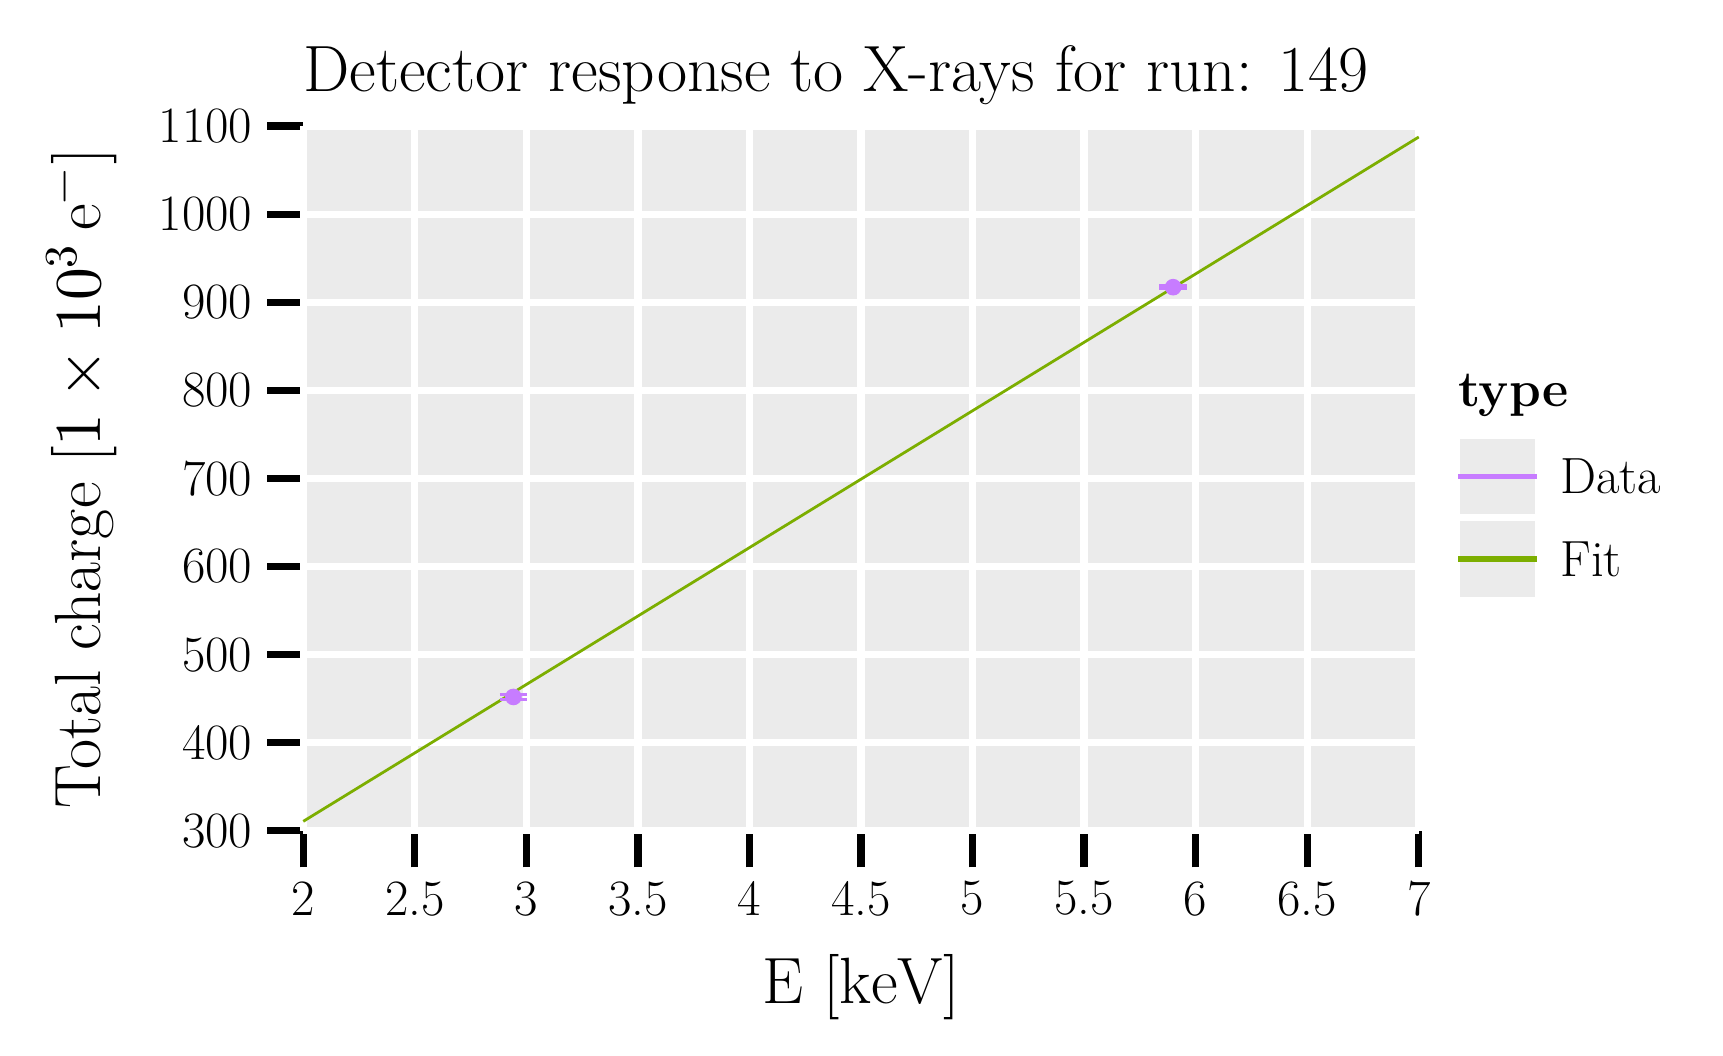
\begin{tikzpicture}[every node/.style={outer sep=0pt, inner sep=0pt}]
\path[use as bounding box] (0, 0) rectangle (600.0bp, 360.0bp) ;
\definecolor{drawColor}{rgb}{0.0, 0.0, 0.0}
\definecolor{fillColor}{rgb}{1.0, 1.0, 1.0}

\draw [color = drawColor, fill = fillColor, draw opacity = 0.0, fill opacity = 1.0, line width = 0.0bp] (0.0000bp, 360.0000bp) rectangle (600.0000bp, 0.0000bp) ;
\node [right, font=\fontsize{23.65409807549184}{28.38491769059021}\selectfont
, anchor=west] at (99.2126bp, 342.9352bp){Detector response to X-rays for run: 149} ;
\definecolor{drawColor}{rgb}{0.0, 0.0, 0.0}
\definecolor{fillColor}{rgb}{0.9200000166893005, 0.9200000166893005, 0.9200000166893005}

\draw [color = drawColor, fill = fillColor, draw opacity = 0.0, fill opacity = 1.0, line width = 0.0bp] (99.2126bp, 324.5669bp) rectangle (500.7874bp, 70.8661bp) ;
\definecolor{drawColor}{rgb}{0.0, 0.0, 0.0}
\definecolor{fillColor}{rgb}{0.0, 0.0, 0.0}

\draw [color = drawColor, fill = fillColor, draw opacity = 1.0, fill opacity = 0.0, line width = 2.628233119499094bp] (99.2126bp, 57.7250bp)--(99.2126bp, 70.8661bp) ;
\draw [color = drawColor, fill = fillColor, draw opacity = 1.0, fill opacity = 0.0, line width = 2.628233119499094bp] (139.3701bp, 57.7250bp)--(139.3701bp, 70.8661bp) ;
\draw [color = drawColor, fill = fillColor, draw opacity = 1.0, fill opacity = 0.0, line width = 2.628233119499094bp] (179.5276bp, 57.7250bp)--(179.5276bp, 70.8661bp) ;
\draw [color = drawColor, fill = fillColor, draw opacity = 1.0, fill opacity = 0.0, line width = 2.628233119499094bp] (219.6850bp, 57.7250bp)--(219.6850bp, 70.8661bp) ;
\draw [color = drawColor, fill = fillColor, draw opacity = 1.0, fill opacity = 0.0, line width = 2.628233119499094bp] (259.8425bp, 57.7250bp)--(259.8425bp, 70.8661bp) ;
\draw [color = drawColor, fill = fillColor, draw opacity = 1.0, fill opacity = 0.0, line width = 2.628233119499094bp] (300.0000bp, 57.7250bp)--(300.0000bp, 70.8661bp) ;
\draw [color = drawColor, fill = fillColor, draw opacity = 1.0, fill opacity = 0.0, line width = 2.628233119499094bp] (340.1575bp, 57.7250bp)--(340.1575bp, 70.8661bp) ;
\draw [color = drawColor, fill = fillColor, draw opacity = 1.0, fill opacity = 0.0, line width = 2.628233119499094bp] (380.3150bp, 57.7250bp)--(380.3150bp, 70.8661bp) ;
\draw [color = drawColor, fill = fillColor, draw opacity = 1.0, fill opacity = 0.0, line width = 2.628233119499094bp] (420.4724bp, 57.7250bp)--(420.4724bp, 70.8661bp) ;
\draw [color = drawColor, fill = fillColor, draw opacity = 1.0, fill opacity = 0.0, line width = 2.628233119499094bp] (460.6299bp, 57.7250bp)--(460.6299bp, 70.8661bp) ;
\draw [color = drawColor, fill = fillColor, draw opacity = 1.0, fill opacity = 0.0, line width = 2.628233119499094bp] (500.7874bp, 57.7250bp)--(500.7874bp, 70.8661bp) ;
\node [font=\fontsize{18.39763183649366}{22.07715820379239}\selectfont
] at (99.2126bp, 46.5549bp){2} ;
\node [font=\fontsize{18.39763183649366}{22.07715820379239}\selectfont
] at (139.3701bp, 46.4348bp){2.5} ;
\node [font=\fontsize{18.39763183649366}{22.07715820379239}\selectfont
] at (179.5276bp, 46.4348bp){3} ;
\node [font=\fontsize{18.39763183649366}{22.07715820379239}\selectfont
] at (219.6850bp, 46.4348bp){3.5} ;
\node [font=\fontsize{18.39763183649366}{22.07715820379239}\selectfont
] at (259.8425bp, 46.5456bp){4} ;
\node [font=\fontsize{18.39763183649366}{22.07715820379239}\selectfont
] at (300.0000bp, 46.4256bp){4.5} ;
\node [font=\fontsize{18.39763183649366}{22.07715820379239}\selectfont
] at (340.1575bp, 46.5641bp){5} ;
\node [font=\fontsize{18.39763183649366}{22.07715820379239}\selectfont
] at (380.3150bp, 46.5641bp){5.5} ;
\node [font=\fontsize{18.39763183649366}{22.07715820379239}\selectfont
] at (420.4724bp, 46.4256bp){6} ;
\node [font=\fontsize{18.39763183649366}{22.07715820379239}\selectfont
] at (460.6299bp, 46.4164bp){6.5} ;
\node [font=\fontsize{18.39763183649366}{22.07715820379239}\selectfont
] at (500.7874bp, 46.6103bp){7} ;
\draw [color = drawColor, fill = fillColor, draw opacity = 1.0, fill opacity = 0.0, line width = 2.628233119499094bp] (99.2126bp, 70.8661bp)--(86.0714bp, 70.8661bp) ;
\draw [color = drawColor, fill = fillColor, draw opacity = 1.0, fill opacity = 0.0, line width = 2.628233119499094bp] (99.2126bp, 102.5787bp)--(86.0714bp, 102.5787bp) ;
\draw [color = drawColor, fill = fillColor, draw opacity = 1.0, fill opacity = 0.0, line width = 2.628233119499094bp] (99.2126bp, 134.2913bp)--(86.0714bp, 134.2913bp) ;
\draw [color = drawColor, fill = fillColor, draw opacity = 1.0, fill opacity = 0.0, line width = 2.628233119499094bp] (99.2126bp, 166.0039bp)--(86.0714bp, 166.0039bp) ;
\draw [color = drawColor, fill = fillColor, draw opacity = 1.0, fill opacity = 0.0, line width = 2.628233119499094bp] (99.2126bp, 197.7165bp)--(86.0714bp, 197.7165bp) ;
\draw [color = drawColor, fill = fillColor, draw opacity = 1.0, fill opacity = 0.0, line width = 2.628233119499094bp] (99.2126bp, 229.4291bp)--(86.0714bp, 229.4291bp) ;
\draw [color = drawColor, fill = fillColor, draw opacity = 1.0, fill opacity = 0.0, line width = 2.628233119499094bp] (99.2126bp, 261.1417bp)--(86.0714bp, 261.1417bp) ;
\draw [color = drawColor, fill = fillColor, draw opacity = 1.0, fill opacity = 0.0, line width = 2.628233119499094bp] (99.2126bp, 292.8543bp)--(86.0714bp, 292.8543bp) ;
\draw [color = drawColor, fill = fillColor, draw opacity = 1.0, fill opacity = 0.0, line width = 2.628233119499094bp] (99.2126bp, 324.5669bp)--(86.0714bp, 324.5669bp) ;
\node [left, font=\fontsize{18.39763183649366}{22.07715820379239}\selectfont
, anchor=east] at (80.8476bp, 70.8661bp){300} ;
\node [left, font=\fontsize{18.39763183649366}{22.07715820379239}\selectfont
, anchor=east] at (80.8476bp, 102.5787bp){400} ;
\node [left, font=\fontsize{18.39763183649366}{22.07715820379239}\selectfont
, anchor=east] at (80.8476bp, 134.2913bp){500} ;
\node [left, font=\fontsize{18.39763183649366}{22.07715820379239}\selectfont
, anchor=east] at (80.8476bp, 166.0039bp){600} ;
\node [left, font=\fontsize{18.39763183649366}{22.07715820379239}\selectfont
, anchor=east] at (80.8476bp, 197.7165bp){700} ;
\node [left, font=\fontsize{18.39763183649366}{22.07715820379239}\selectfont
, anchor=east] at (80.8476bp, 229.4291bp){800} ;
\node [left, font=\fontsize{18.39763183649366}{22.07715820379239}\selectfont
, anchor=east] at (80.8476bp, 261.1417bp){900} ;
\node [left, font=\fontsize{18.39763183649366}{22.07715820379239}\selectfont
, anchor=east] at (80.8476bp, 292.8543bp){1000} ;
\node [left, font=\fontsize{18.39763183649366}{22.07715820379239}\selectfont
, anchor=east] at (80.8476bp, 324.5669bp){1100} ;
\node [font=\fontsize{23.65409807549184}{28.38491769059021}\selectfont
] at (300.0000bp, 14.6691bp){E [$\si{keV}$]} ;
\node [rotate = 90.0, font=\fontsize{23.65409807549184}{28.38491769059021}\selectfont
] at (19.4033bp, 197.7165bp){Total charge [$\SI{1e3}{e^-}$]} ;
\definecolor{drawColor}{rgb}{1.0, 1.0, 1.0}
\definecolor{fillColor}{rgb}{0.0, 0.0, 0.0}

\draw [color = drawColor, fill = fillColor, draw opacity = 1.0, fill opacity = 0.0, line width = 2.628233119499094bp] (99.2126bp, 324.5669bp)--(99.2126bp, 70.8661bp) ;
\draw [color = drawColor, fill = fillColor, draw opacity = 1.0, fill opacity = 0.0, line width = 2.628233119499094bp] (139.3701bp, 324.5669bp)--(139.3701bp, 70.8661bp) ;
\draw [color = drawColor, fill = fillColor, draw opacity = 1.0, fill opacity = 0.0, line width = 2.628233119499094bp] (179.5276bp, 324.5669bp)--(179.5276bp, 70.8661bp) ;
\draw [color = drawColor, fill = fillColor, draw opacity = 1.0, fill opacity = 0.0, line width = 2.628233119499094bp] (219.6850bp, 324.5669bp)--(219.6850bp, 70.8661bp) ;
\draw [color = drawColor, fill = fillColor, draw opacity = 1.0, fill opacity = 0.0, line width = 2.628233119499094bp] (259.8425bp, 324.5669bp)--(259.8425bp, 70.8661bp) ;
\draw [color = drawColor, fill = fillColor, draw opacity = 1.0, fill opacity = 0.0, line width = 2.628233119499094bp] (300.0000bp, 324.5669bp)--(300.0000bp, 70.8661bp) ;
\draw [color = drawColor, fill = fillColor, draw opacity = 1.0, fill opacity = 0.0, line width = 2.628233119499094bp] (340.1575bp, 324.5669bp)--(340.1575bp, 70.8661bp) ;
\draw [color = drawColor, fill = fillColor, draw opacity = 1.0, fill opacity = 0.0, line width = 2.628233119499094bp] (380.3150bp, 324.5669bp)--(380.3150bp, 70.8661bp) ;
\draw [color = drawColor, fill = fillColor, draw opacity = 1.0, fill opacity = 0.0, line width = 2.628233119499094bp] (420.4724bp, 324.5669bp)--(420.4724bp, 70.8661bp) ;
\draw [color = drawColor, fill = fillColor, draw opacity = 1.0, fill opacity = 0.0, line width = 2.628233119499094bp] (460.6299bp, 324.5669bp)--(460.6299bp, 70.8661bp) ;
\draw [color = drawColor, fill = fillColor, draw opacity = 1.0, fill opacity = 0.0, line width = 2.628233119499094bp] (500.7874bp, 324.5669bp)--(500.7874bp, 70.8661bp) ;
\draw [color = drawColor, fill = fillColor, draw opacity = 1.0, fill opacity = 0.0, line width = 2.628233119499094bp] (99.2126bp, 70.8661bp)--(500.7874bp, 70.8661bp) ;
\draw [color = drawColor, fill = fillColor, draw opacity = 1.0, fill opacity = 0.0, line width = 2.628233119499094bp] (99.2126bp, 102.5787bp)--(500.7874bp, 102.5787bp) ;
\draw [color = drawColor, fill = fillColor, draw opacity = 1.0, fill opacity = 0.0, line width = 2.628233119499094bp] (99.2126bp, 134.2913bp)--(500.7874bp, 134.2913bp) ;
\draw [color = drawColor, fill = fillColor, draw opacity = 1.0, fill opacity = 0.0, line width = 2.628233119499094bp] (99.2126bp, 166.0039bp)--(500.7874bp, 166.0039bp) ;
\draw [color = drawColor, fill = fillColor, draw opacity = 1.0, fill opacity = 0.0, line width = 2.628233119499094bp] (99.2126bp, 197.7165bp)--(500.7874bp, 197.7165bp) ;
\draw [color = drawColor, fill = fillColor, draw opacity = 1.0, fill opacity = 0.0, line width = 2.628233119499094bp] (99.2126bp, 229.4291bp)--(500.7874bp, 229.4291bp) ;
\draw [color = drawColor, fill = fillColor, draw opacity = 1.0, fill opacity = 0.0, line width = 2.628233119499094bp] (99.2126bp, 261.1417bp)--(500.7874bp, 261.1417bp) ;
\draw [color = drawColor, fill = fillColor, draw opacity = 1.0, fill opacity = 0.0, line width = 2.628233119499094bp] (99.2126bp, 292.8543bp)--(500.7874bp, 292.8543bp) ;
\draw [color = drawColor, fill = fillColor, draw opacity = 1.0, fill opacity = 0.0, line width = 2.628233119499094bp] (99.2126bp, 324.5669bp)--(500.7874bp, 324.5669bp) ;
\definecolor{drawColor}{rgb}{0.4848798215389252, 0.683388352394104, 0.0}
\definecolor{fillColor}{rgb}{0.0, 0.0, 0.0}

\draw [color = drawColor, fill = fillColor, draw opacity = 1.0, fill opacity = 0.0, line width = 1.0bp]
(99.2126bp, 74.2733bp)  -- 
(103.2689bp, 76.7618bp)  -- 
(107.3252bp, 79.2503bp)  -- 
(111.3815bp, 81.7388bp)  -- 
(115.4378bp, 84.2273bp)  -- 
(119.4942bp, 86.7158bp)  -- 
(123.5505bp, 89.2043bp)  -- 
(127.6068bp, 91.6928bp)  -- 
(131.6631bp, 94.1813bp)  -- 
(135.7194bp, 96.6698bp)  -- 
(139.7757bp, 99.1583bp)  -- 
(143.8320bp, 101.6468bp)  -- 
(147.8883bp, 104.1354bp)  -- 
(151.9446bp, 106.6239bp)  -- 
(156.0010bp, 109.1124bp)  -- 
(160.0573bp, 111.6009bp)  -- 
(164.1136bp, 114.0894bp)  -- 
(168.1699bp, 116.5779bp)  -- 
(172.2262bp, 119.0664bp)  -- 
(176.2825bp, 121.5549bp)  -- 
(180.3388bp, 124.0434bp)  -- 
(184.3951bp, 126.5319bp)  -- 
(188.4514bp, 129.0204bp)  -- 
(192.5078bp, 131.5089bp)  -- 
(196.5641bp, 133.9975bp)  -- 
(200.6204bp, 136.4860bp)  -- 
(204.6767bp, 138.9745bp)  -- 
(208.7330bp, 141.4630bp)  -- 
(212.7893bp, 143.9515bp)  -- 
(216.8456bp, 146.4400bp)  -- 
(220.9019bp, 148.9285bp)  -- 
(224.9582bp, 151.4170bp)  -- 
(229.0146bp, 153.9055bp)  -- 
(233.0709bp, 156.3940bp)  -- 
(237.1272bp, 158.8825bp)  -- 
(241.1835bp, 161.3710bp)  -- 
(245.2398bp, 163.8595bp)  -- 
(249.2961bp, 166.3481bp)  -- 
(253.3524bp, 168.8366bp)  -- 
(257.4087bp, 171.3251bp)  -- 
(261.4650bp, 173.8136bp)  -- 
(265.5214bp, 176.3021bp)  -- 
(269.5777bp, 178.7906bp)  -- 
(273.6340bp, 181.2791bp)  -- 
(277.6903bp, 183.7676bp)  -- 
(281.7466bp, 186.2561bp)  -- 
(285.8029bp, 188.7446bp)  -- 
(289.8592bp, 191.2331bp)  -- 
(293.9155bp, 193.7216bp)  -- 
(297.9718bp, 196.2102bp)  -- 
(302.0282bp, 198.6987bp)  -- 
(306.0845bp, 201.1872bp)  -- 
(310.1408bp, 203.6757bp)  -- 
(314.1971bp, 206.1642bp)  -- 
(318.2534bp, 208.6527bp)  -- 
(322.3097bp, 211.1412bp)  -- 
(326.3660bp, 213.6297bp)  -- 
(330.4223bp, 216.1182bp)  -- 
(334.4786bp, 218.6067bp)  -- 
(338.5350bp, 221.0952bp)  -- 
(342.5913bp, 223.5837bp)  -- 
(346.6476bp, 226.0722bp)  -- 
(350.7039bp, 228.5608bp)  -- 
(354.7602bp, 231.0493bp)  -- 
(358.8165bp, 233.5378bp)  -- 
(362.8728bp, 236.0263bp)  -- 
(366.9291bp, 238.5148bp)  -- 
(370.9854bp, 241.0033bp)  -- 
(375.0418bp, 243.4918bp)  -- 
(379.0981bp, 245.9803bp)  -- 
(383.1544bp, 248.4688bp)  -- 
(387.2107bp, 250.9573bp)  -- 
(391.2670bp, 253.4458bp)  -- 
(395.3233bp, 255.9343bp)  -- 
(399.3796bp, 258.4228bp)  -- 
(403.4359bp, 260.9114bp)  -- 
(407.4922bp, 263.3999bp)  -- 
(411.5486bp, 265.8884bp)  -- 
(415.6049bp, 268.3769bp)  -- 
(419.6612bp, 270.8654bp)  -- 
(423.7175bp, 273.3539bp)  -- 
(427.7738bp, 275.8424bp)  -- 
(431.8301bp, 278.3309bp)  -- 
(435.8864bp, 280.8194bp)  -- 
(439.9427bp, 283.3079bp)  -- 
(443.9990bp, 285.7964bp)  -- 
(448.0554bp, 288.2849bp)  -- 
(452.1117bp, 290.7735bp)  -- 
(456.1680bp, 293.2620bp)  -- 
(460.2243bp, 295.7505bp)  -- 
(464.2806bp, 298.2390bp)  -- 
(468.3369bp, 300.7275bp)  -- 
(472.3932bp, 303.2160bp)  -- 
(476.4495bp, 305.7045bp)  -- 
(480.5058bp, 308.1930bp)  -- 
(484.5622bp, 310.6815bp)  -- 
(488.6185bp, 313.1700bp)  -- 
(492.6748bp, 315.6585bp)  -- 
(496.7311bp, 318.1470bp)  -- 
(500.7874bp, 320.6355bp)
;\definecolor{drawColor}{rgb}{0.7804079055786133, 0.4866028726100922, 1.0}
\definecolor{fillColor}{rgb}{0.0, 0.0, 0.0}

\draw [color = drawColor, fill = fillColor, draw opacity = 1.0, fill opacity = 0.0, line width = 1.0bp] (174.8693bp, 120.0437bp)--(174.8693bp, 118.0718bp) ;
\draw [color = drawColor, fill = fillColor, draw opacity = 1.0, fill opacity = 0.0, line width = 1.0bp] (169.8693bp, 120.0437bp)--(179.8693bp, 120.0437bp) ;
\draw [color = drawColor, fill = fillColor, draw opacity = 1.0, fill opacity = 0.0, line width = 1.0bp] (169.8693bp, 118.0718bp)--(179.8693bp, 118.0718bp) ;
\draw [color = drawColor, fill = fillColor, draw opacity = 1.0, fill opacity = 0.0, line width = 1.0bp] (412.3606bp, 267.0456bp)--(412.3606bp, 266.1008bp) ;
\draw [color = drawColor, fill = fillColor, draw opacity = 1.0, fill opacity = 0.0, line width = 1.0bp] (407.3606bp, 267.0456bp)--(417.3606bp, 267.0456bp) ;
\draw [color = drawColor, fill = fillColor, draw opacity = 1.0, fill opacity = 0.0, line width = 1.0bp] (407.3606bp, 266.1008bp)--(417.3606bp, 266.1008bp) ;
\definecolor{drawColor}{rgb}{0.0, 0.0, 0.0}
\definecolor{fillColor}{rgb}{0.7804079055786133, 0.4866028726100922, 1.0}

\draw [color = drawColor, fill = fillColor, draw opacity = 0.0, fill opacity = 1.0, line width = 1.0bp] (174.8693bp, 119.0577bp) circle [radius=3.0bp] ;
\draw [color = drawColor, fill = fillColor, draw opacity = 0.0, fill opacity = 1.0, line width = 1.0bp] (412.3606bp, 266.5732bp) circle [radius=3.0bp] ;
\node [right, font=\fontsize{18.39763183649366}{22.07715820379239}\selectfont
, anchor=west] at (514.9606bp, 227.4803bp){\textbf{type}
} ;
\definecolor{drawColor}{rgb}{1.0, 1.0, 1.0}
\definecolor{fillColor}{rgb}{0.9200000166893005, 0.9200000166893005, 0.9200000166893005}

\draw [color = drawColor, fill = fillColor, draw opacity = 1.0, fill opacity = 1.0, line width = 1.0bp] (514.9606bp, 212.5984bp) rectangle (543.3071bp, 184.2520bp) ;
\definecolor{drawColor}{rgb}{0.7804079055786133, 0.4866028726100922, 1.0}
\definecolor{fillColor}{rgb}{0.0, 0.0, 0.0}

\draw [color = drawColor, fill = fillColor, draw opacity = 1.0, fill opacity = 0.0, line width = 2.0bp] (514.9606bp, 198.4252bp)--(543.3071bp, 198.4252bp) ;
\node [right, font=\fontsize{18.39763183649366}{22.07715820379239}\selectfont
, anchor=west] at (551.8110bp, 198.4252bp){Data} ;
\definecolor{drawColor}{rgb}{1.0, 1.0, 1.0}
\definecolor{fillColor}{rgb}{0.9200000166893005, 0.9200000166893005, 0.9200000166893005}

\draw [color = drawColor, fill = fillColor, draw opacity = 1.0, fill opacity = 1.0, line width = 1.0bp] (514.9606bp, 182.8346bp) rectangle (543.3071bp, 154.4882bp) ;
\definecolor{drawColor}{rgb}{0.4848798215389252, 0.683388352394104, 0.0}
\definecolor{fillColor}{rgb}{0.0, 0.0, 0.0}

\draw [color = drawColor, fill = fillColor, draw opacity = 1.0, fill opacity = 0.0, line width = 2.0bp] (514.9606bp, 168.6614bp)--(543.3071bp, 168.6614bp) ;
\node [right, font=\fontsize{18.39763183649366}{22.07715820379239}\selectfont
, anchor=west] at (551.8110bp, 168.6614bp){Fit} ;

\end{tikzpicture}

\end{document}

